\documentclass{article}
\usepackage[utf8]{inputenc}
\usepackage{amsmath}
\usepackage{graphicx}
\usepackage[procnames]{listings}
\usepackage{color}
\usepackage{indentfirst}
\usepackage{xcolor}
\usepackage{sectsty}
\usepackage[explicit]{titlesec}
\usepackage[normalem]{ulem}
\usepackage[hidelinks]{hyperref}

\usepackage{geometry}
 \geometry{
 a4paper,
 %total={170mm,257mm},
 left=20mm,
 %top=20mm,
 }
\title{\textbf{ UML Diagrams}}

\author{}
\date{}

\begin{document}


\maketitle
\begin{center}

\includegraphics[scale=0.6]{images/logoLIS_modified.jpg}
\\
\textbf{LIBRERIA}\\
LIBRARY INFORMATION SYSTEM\\
%\vspace{2 cm}
Group Number : 52\\
Group members: \\
\begin{itemize}
\item \begin{center}Ashrujit Ghoshal (14CS10060)\end{center}
\item \begin{center}Sayan Ghosh (14CS10061)\end{center}
\end{itemize}

\end{center}
\newpage
%\clearpage
\hypertarget{toc}{}
\tableofcontents
\newpage

\section{Use Case Diagram}

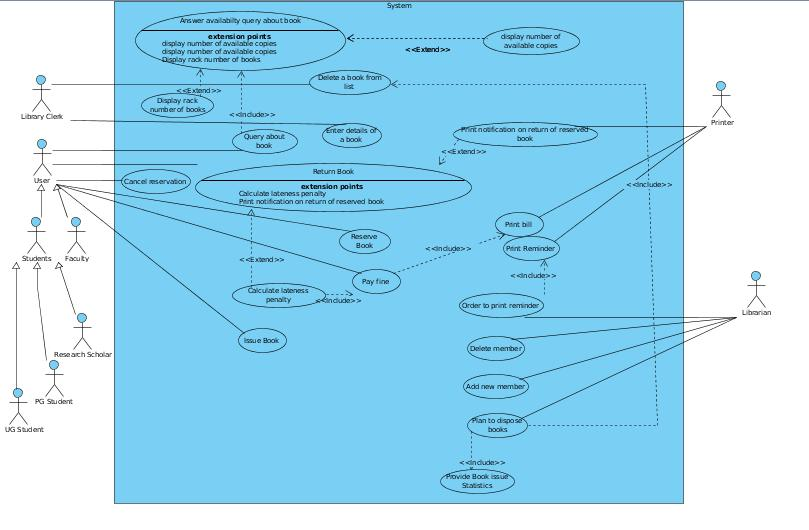
\includegraphics[scale=0.55]{images/useCaseDiag.jpg}\\
\subsubsection*{Use case of User :}
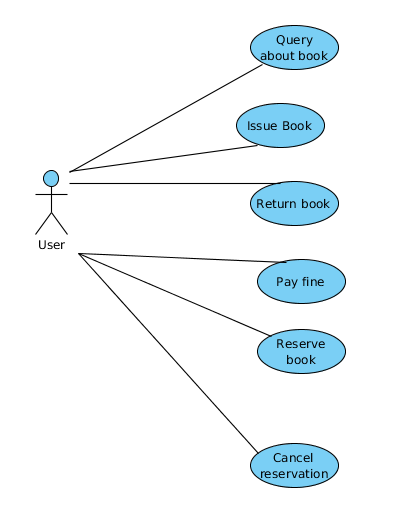
\includegraphics[scale=0.6]{images/userCaseDiag.png}\\
\subsubsection*{Use case of Library Clerk :}
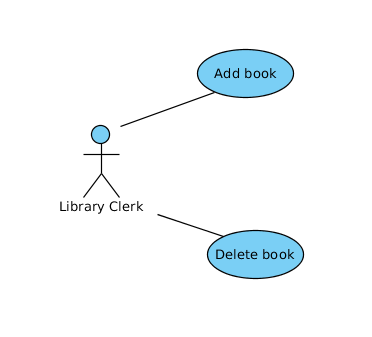
\includegraphics[scale=0.6]{images/clerkClassDiag.png}\\
\subsubsection*{Use case of Librarian :}
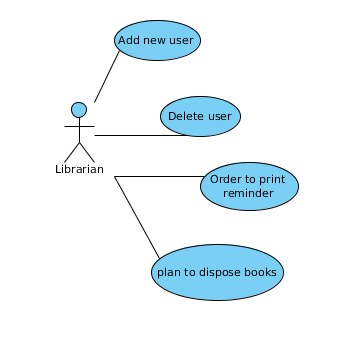
\includegraphics[scale=0.6]{images/librarianCaseDiag.png}\\
Description :
\\
\begin{enumerate}
\item User use cases:
	\begin{itemize}
	
	\item Query about Book\\
	\begin{itemize}
	\item Preconditions:\\
	1. The user must be logged in .\\
	2.The book must exist in the library\\
\item  Postcondition: \\If the book exists in the library,the availablity status of the book is returned\\
 \item Failure Situations:\\ The library does not have  the book \\
 \item Postcondition in case of failure:\\A message to user about the same\\
\item  Actors:\\ User communicates with the system\\
\item  Trigger:\\ User chooses the option to search books\\
 \item Main Success Scenario: \\The library has a copy of the book and it is available for issue.\\
\item  Extensions/Variations: \\The library has a copy of the book but currently none of the copies are available.The book maybe reserved by the user.
	\end{itemize}
 \item Issue Book\\
	\begin{itemize}
	 \item Preconditions:\\
	 1. The user must be logged in .\\
	 2.The book must exist in the library \\
	 3.It must be available for issue.\\
	 4.The user must not have exhausted his quota of number of books\\
 \item Postcondition:\\After successful issue the user account is updated\\
 \item Failure Situations:\\
 1. The library does not have  the book\\ 
 2.The library has the book and it is not avaiable for issue.\\
 3.The user has exhausted his quota of maximum number of books\\
 \item Postcondition in case of failure:\\In failure case 2. the user may choose to reserve the book if he has not exhausted his quota\\
 \item Actors:\\ User communicates with the system\\
 \item Trigger: \\User chooses the option to issue books\\
 \item Main Success Scenario:\\ The library has a copy of the book and it is available for issue.
	\end{itemize}
 

 \item Return Book\\
 \begin{itemize}
 \item Precondition:\\
 1.User must be logged in.\\
 2.User must have previously issued the book.\\
 \item Postcondition:\\
 1.If the book was overdue the penalty is calculated and a bill is printed\\ 
 2.In case the book was reserved by some other user, a notification is sent out to the other user.\\
 3.The user account is updated\\
 \item Failure Situations:\\The user has not issued any book\\
 \item Postcondition in case of failure:\\A message is give to the user about the same\\
 \item Actors:\\ User communicates with the system\\
 \item Trigger:\\ User chooses the option to return issued books\\
\item  Main Success Scenario: \\The user had previously issued the book\\
 \end{itemize}
 
 \item Reserve Book\\
	\begin{itemize}
	\item  Preconditions:\\
	1. The user must be logged in .\\
	2.The book must exist in the library\\ 
	3.It must not  be available for issue.\\
	4.The user must not have exhausted his quota of number of books\\
 \item Postcondition:\\
 1.After successful issue the user account is updated \\
 2.When the book is returned a notification is sent to the user.\\
 \item Failure Situations:\\
 1. The library does not have  the book \\
 2.The library has the book and it is  avaiable for issue.\\
 3.The user has exhausted his quota of maximm number of books\\
 \item Postcondition in case of failure:\\In failure case 2. the user may choose to issue the book if he has not exhausted his quota\\
 \item Actors:\\ User communicates with the system\\
 \item Trigger:\\ User chooses the option to reserve book\\
 \item Main Success Scenario:\\ The library has a copy of the book and it is not available for issue.\\
 
	\end{itemize}
 
 \item Cancel Reservation\\
 \begin{itemize}
 \item  Preconditions:\\
 1. The user must be logged in .\\
 2.The user must have reserved the book\\
 \item Postcondition:\\
 1.After successful issue the user account is updated \\
Failure Situations:\\The user has not issued any book\\
 \item Actors: \\User communicates with the system\\
 \item Trigger:\\ 
 1.User chooses the option to cancel reservation of a book \\
 2.User does not issue the reserved book within 7 days of return\\
 \item Main Success Scenario:\\ The library has a copy of the book and the user must have reserved it previously\\
	
 \end{itemize}

\item Pay Fine\\
	\begin{itemize}
	\item  Precondition:\\
	\begin{enumerate}	
	\item User must be logged in.\\
	\item User must have previously issued the book.\\The book must be overdue\\
	\end{enumerate}
 \item Postcondition:\\
  The book was overdue the penalty is calculated and a bill is printed 
 \item Failure Situations:
 \begin{enumerate}
 \item The user has not issued any book
  \item No returned books are overdue
	\end{enumerate} 
 \item Actors: User communicates with the system
 \item Trigger: User chooses the option to return issued books
 \item Main Success Scenario: The user had previously issued the book and the book is overdue
	\end{itemize}
\end{itemize}


\item Library Clerk Use Cases
 \begin{itemize}
 \item Enter details of a book
 \begin{itemize}
 \item Preconditions:1. The clerk must be logged in.\\2.The book must not be previously entered in the system
 \item Failure Situations:\\ The book is already in the system
 \item Postcondition in case of failure:\\A message to clerk about the same
 \item Actors:\\ library clerk communicates with the system
 \item Trigger:\\ Clerk chooses the option to enter new books
 \item Main Success Scenario:\\ The library  does not have the book and the book is newly entered in the system
\item  Extensions/Variations:\\ The library hasthe book and the umber of copies is increased
\end{itemize}
 \item Delete a book 
 \begin{itemize}
	\item 	Preconditions:\\1. The clerk must be logged in.\\2.The book must  be previously entered in the system \\3.The librarian has decided to dispose the book\\
 \item Failure Situations:\\ The book is not in the system\\
 \item Postcondition in case of failure:\\A message to clerk about the same\\
 \item Actors:\\ library clerk communicates with the system\\
 \item Trigger:\\ Clerk chooses the option to delete books\\
 \item Main Success Scenario:\\ The library  has the book and it is removed from the system.\\
 \item Extensions/Variations: \\The library has the book and the number of copies is reduced.\\
 
\end{itemize}	 
 
 \end{itemize}
 


\item Librarian Use Cases:
\begin{itemize}
 \item Add new member
 \begin{itemize}
  \item Preconditions:1.Librarian must be logged in\\2. A person must apply for membership
 \\ \item Postcondition:\\A new member account is created \\
 \item Failure Situations:\\ The user is already registered\\
 \item Postcondition in case of failure:\\A message to librarian about the same\\
\item  Actors:\\ Librarian communicates with the system\\
 \item Trigger: \\Librarian  chooses the option to add member\\
 \item Main Success Scenario:\\ The user is not previously registered\\
 \end{itemize}

\item Delete member\\ 
 \begin{itemize}
  \item Preconditions:\\ 1.Librarian must be logged in\\ 2. A person must apply for cacellation membership\\ 
 \item Postcondition:\\ The member account is deleted\\ 
 \item Failure Situations: \\ The user has no account\\ 
 \item Postcondition in case of failure:\\ A message to librarian about the same\\ 
 \item Actors: \\ Librarian communicates with the system\\ 
 \item Trigger:\\  Librarian  chooses the option to delete member\\ 
 \item Main Success Scenario:\\  The user   previously has an account\\ 
 \end{itemize}
 
 \item Order to print reminder\\ 
 \begin{itemize}
  \item Preconditions:\\ 1.Librarian must be logged in\\ 2. A book issued by a member must be overdue\\ 
 \item Postcondition:\\ A message is sent to the user.\\ 
 \item Failure Situations:\\  There are no overdue books\\ 
 \item Postcondition in case of failure:\\ A message to librarian about the same\\ 
 \item Actors: \\ Librarian communicates with the system\\ 
 \item Trigger:\\  Librarian  chooses the option to print reminder\\ 
 \item Main Success Scenario :\\  There are some overdue books\\ 
 \end{itemize}

\item Plan to dispose books\\ 
 \begin{itemize}
  \item Preconditions:\\ 1.Librarian must be logged in\\ 2. The book must not have been issued even once for 5 years\\ 
 \item Postcondition:\\ The book is disposed with a message to the library clerk to delete it.\\ 
 \item Actors:\\  Librarian communicates with the system\\ 
 \item Trigger:\\  Librarian  chooses the option to dispose book\\ 
 \item Main Success Scenario:\\  The book has not been issue for 5 years\\ 
 \end{itemize}
 

\end{itemize}

\item System Use Cases:\\ 
 \begin{itemize}
 
  \item Answer availibilty Query about Book\\ 
	\begin{itemize}
	\item  Preconditions:\\ 1.An user makes a query\\ 
 \item Postcondition: \\ If the book is available, use cases display rack number and number of copies are called\\ 
 \item Actors:\\  System communicates with the user\\ 
 \item Trigger: \\ User chooses the option to search books\\ 
	\end{itemize}

\item Display rack number of book\\ 
	\begin{itemize}
	\item  Preconditions:\\ 1.If the book is available the use case answer availibility query invokes this\\ 
 \item Postcondition:\\  Rack numbers are displayed\\ 
 \item Actors:\\  System communicates with the user\\ 
 \item Trigger:\\  answer availibity query triggers this\\ 
	\end{itemize}
 
 \item Display number of copies of book\\ 
	\begin{itemize}
	\item  Preconditions:\\ 1.If the book is available the use case answer availibility query invokes this\\ 
 \item Postcondition:\\  the number of copies of a book are displayed\\ 
 \item Actors: \\ System communicates with the user\\ 
 \item Trigger:\\  answer availibity query triggers this\\ 
	\end{itemize}

\item Calculate lateness penalty\\ 
	\begin{itemize}
	\item  Preconditions:\\ 1.If the book is overdue, return book invokes this\\ 
 \item Postcondition:\\ Penalty is calculated and print bill is invoked\\ 
 \item Actors: \\ System communicates with the user\\ 
 \item Trigger: \\ return book query triggers this\\ 
	\end{itemize}
 
 \item Provide book issue statistics
	\begin{itemize}
	\item  Preconditions:\\ 1.The use case is invoked by plan to dispose books\\ 
 \item Postcondition:\\ Statistics of books is displayed\\ 
 \item Actors: \\ system communicates with librarian\\ 
 \item Trigger:\\ Plan dispose book is invoked\\ 
	\end{itemize}

 \end{itemize}
\item Printer use cases:\\ 
\begin{itemize}
\item Print bill of penalty\\ 
\begin{itemize}
\item Preconditions:\\ Some user must have returned the issued book later than his designated return date.\\ 
 \item Postcondition:\\ Bill of penalty is printed\\ 
 \item Actors:\\  Printer communicates with the system\\ 
 \item Trigger:\\  Calculate lateness penalty triggers print bill\\ 
\end{itemize}

\item Print reminder\\ 
\begin{itemize}
\item  Preconditions:\\ Some user must have exceeded the due date\\ 
 \item Postcondition:\\ Reminder to user is printed\\ 
 \item Actors:\\  Printer communicates with the system\\ 
 \item Trigger:\\ order to print reminder triggers this\\ 
\end{itemize}

\item Print notification on return of reserved book\\ 
\begin{itemize}
\item Preconditions:\\ Some user must have returned a reserved book \\ 
 \item Postcondition:\\ A notification is printed to the user who reserved the book\\ 
 \item Actors: \\ Printer communicates with the system which communicates with user\\ 
 \item Trigger:\\ return book may trigger this use case\\ 
\end{itemize}

\end{itemize}
\end{enumerate}

\section{Class Diagrams}
\subsection*{Initial Draft}
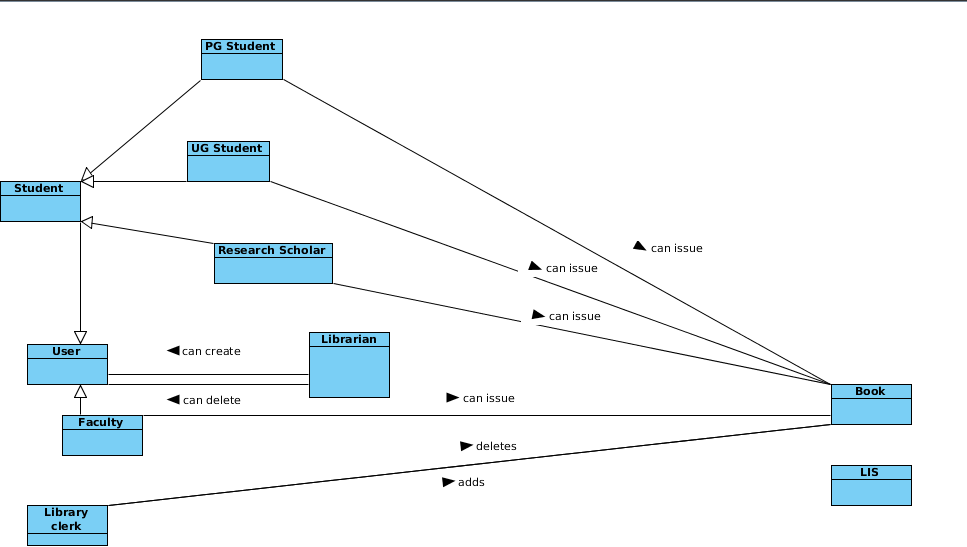
\includegraphics[scale=0.35]{images/classDiagNaive.png}\\
\\
\subsection*{Final Draft}
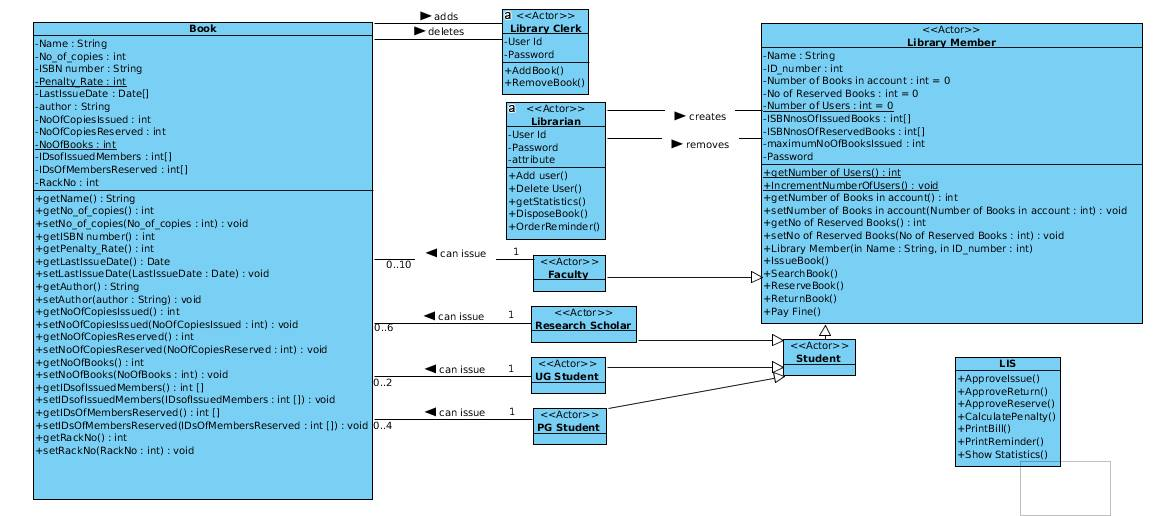
\includegraphics[scale=0.35]{images/classDiagFinal.jpg}


Description : \\

\begin{itemize}
\item Book
\begin{itemize}
\item Class Attributes:\\
\\Name:Store the name of book
\\No$\_$of$\_$copies:Stores the number of copies of a book
\\Penalty$\_$Rate:the rate of penalty for book.A static member as it is common for all the books
\\Author:stores name  author of book 
\\LastIssueDateDate:Stores the last issued date of book
\\NoOfCopiesIssued:Stores the number of copies of the book that have been issued out
\\NoOfCopiesReserved:Stores the number of issued books that have been reserved
\\NoOfBooks:A static variable storing the total number of books
\\IDsofIssuedMembers[]:An array of integers storing the ids of all the members who have issued copies of the book
\\IDsOfMembersReserved[]:An array of integers storing the ids of all the members who have issued copies of the book
\\RackNo:stores the rack number where the book is kept

\item Operations:
\\Getter functions for name,No$\_$of$\_$copies,ISBN number,Penalty$\_$rate,LastIssueDate,author,NoOfCopiesIssued,NoOfCopiesReserved,NoOfBooks,IDsofIssuedMembers,IDsOfMembersReserved,RackNo.

We have used getters for these as we need to view these attributes from outside 
\\
Setters for No$\_$of$\_$copies,LastIssueDate,NoOfCopiesIssued,NoOfCopiesReserved,IDsOfIssuedMembers, IDSOfMembersReserved,RackNo.

We have used setters for these as these are changeable with time and need to be changesd at a later point of time.These being private members setters ar only way to modify them
\end{itemize}


\item Library Member 
\begin{itemize}
\item Attributes:
\begin{itemize}
\item Name:Name of the user
\item ID$\_$number:Login id of the user
\item Number of books in account:Total number of issued books
\item Number of reserved books:Total number of books issued by the user
\item NoOfUsers:A static variable storuing total number of users
\item ISBNnosOfIssuedBooks[]:an array storing the ISBN number of all books issued by the user
\item ISBNnosOfReservedBooks[]:an array storing the ISBN number of all books reserved by the user
\item maximumNoOfBooksIssued:the maximum number of books that the user can issue
\item Pasword:The login password of the user which is necessary for login authentication
\end{itemize}

\item Operations:
\begin{itemize}

\item Constructor to initialize member\\
\item Getters for NumberOfBooksinAccount,No ofReservedBooks,NoOfUsers.
We have used getters for these as we need to view these attributes from outside \\\
\item Setters for NumberOfUsers,Number of books in account,No Of reserved Books.


We have used setters for these as these are changeable with time and need to be changesd at a later point of time.These being private members setters ar only way to modify them
\\
\item IssueBook:called when member tries to issue a book\\
\item SearchBook:Called when member tries to search fo a book\\
\item Reserve Book:Called when member tries to reserve a book\\
\item ReturnBook:called when member tries to return a book\\
\item PayFine:Called when member returns an overdue book\\

\end{itemize}
\end{itemize}

\item Library Clerk
\begin{itemize}
\item Attributes:
\begin{itemize}
\item UserId:User Id of the library Clerk\\
\item Password:Password of the library Clerk\\
\end{itemize}

\item Operations:
\begin{itemize}
\item AddBook:Adds a new procured book to database\\
\item Removebook:Deletes a disposed book from database\\
\end{itemize}
\end{itemize}
\item Librarian

\begin{itemize}

\item Attributes:
\begin{itemize}
\item UserId:User Id of the librarian
\item Password:Password of the librarian
\end{itemize}
\item Operations:
\begin{itemize}
\item AddUser:Adds a new user account
\item DeleteUser:Deletes an existing user account
\item getStatistics: asks for statistics from LIS
\item DisposeBooks:Disposes a book not issued in 5 years
\item OrderReminder:Orders LIS to print reminder on overdue books
\end{itemize}
\end{itemize}

\item LIS
\begin{itemize}
\item Operations:\\
\begin{itemize}

\item ApproveIssue:Called when user tries to issue a book
\item ApproveReturn:Called when user tries to return a book

\item ApproveReserve:Called when user tries to reserve a book
\item CalculatePenalty:Calculates penalty on overdue book
\item PrintBill:prints penalty Bill
\item PrintReminder:prints Reminder on overdue books
\item Show Statistics:Display statistics of books issued

\end{itemize}
\end{itemize}

\item Faculty\\
It is a generalization of Library User
\item Student\\
It is a generalization of Library User
\item Research Scholar\\
It is a generalization of Student
\item UG Student\\
It is a generalization of Student
\item PG Student\\
It is a generalization of Student

\end{itemize}

\section{Sequence Diagram}
\subsubsection*{Add User Sequence Diagram}
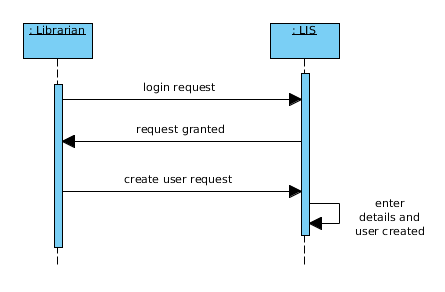
\includegraphics[scale=0.50]{images/seqDiagAddUser.png}
\\
Description : The user needs to login succesfully into the account as the librarian as he/she only has the priviledge to add a user .He then provides the suitable details required to create a user in the library and creates it.
\\

\subsubsection*{Remove User Sequence Diagram}
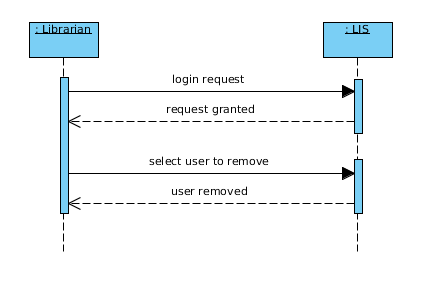
\includegraphics[scale=0.50]{images/seqDiagRemoveUser.png}
\\
Description : The user needs to login succesfully into the account as the librarian as he/she only has the priviledge to remove a user .He then provides the suitable details required to remove a user in the library and the user along with all the user history is removed from the library database.
\\

\subsubsection*{Add book Sequence Diagram}
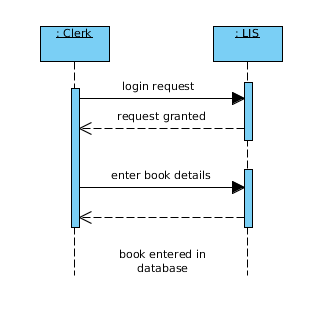
\includegraphics[scale=0.50]{images/seqDiagAddBook.png}
\\
Description : The user needs to login succesfully into the account as the library clerk as he/she only has the priviledge to add a book into the database of the library.The clerk then provides the suitable details of the book into the system and it automatically updates this into the database at the same time. The book will then be available for issuing ad reservation by the members.
\\

\subsubsection*{Remove book Sequence Diagram}
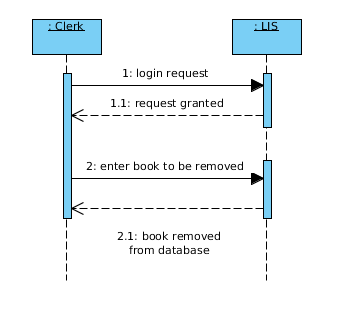
\includegraphics[scale=0.50]{images/seqDiagBookRemoval.png}
\\
The user needs to succesfully login as the library clerk as he/she only has the priviledge to remove a book from the sytem if he/she feels that the book has been unused for a long period of time and is not required anymore.The user feeds the details of the book to be removed and the system automatically removes all the records related to this book from the system and will not be thereafter available for issuing and reservation by the other library members/users.
\\

\subsubsection*{Issue book Sequence Diagram}
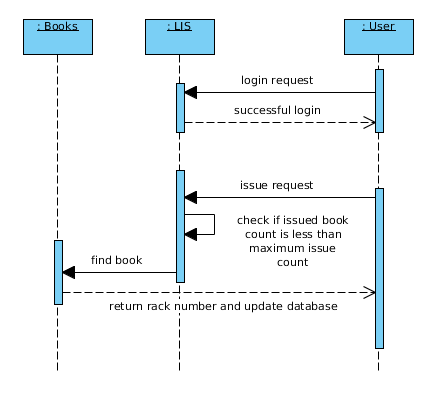
\includegraphics[scale=0.50]{images/seqDiagIssueBook.png}
\\
The user needs to succesfully login as a valid member or user of the library to issue a book. Also the book must be available in the library at that instant and also he/she must not exceed the maximum book count against his/her account in the library.The book is then added into the user's account and is thus issued.\\

\subsubsection*{Return book Sequence Diagram}
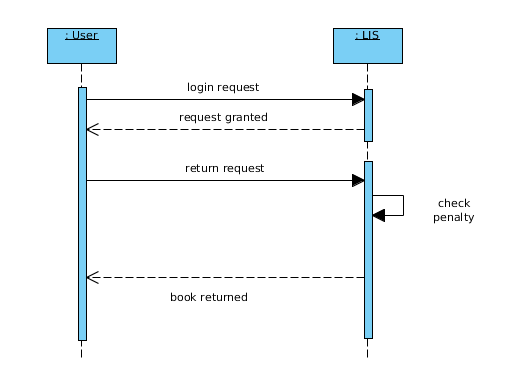
\includegraphics[scale=0.50]{images/seqDiagReturnBook.png}
\\
The user needs to successfully login as a valid member of the library to avail the option of returning the book.The book should not be overdue else the user has to pay a fine as per the rate predecided by the library authority. The book in any case is returned and all changes are updated in the user details of the database.
\\

\subsubsection*{Search book Sequence Diagram}
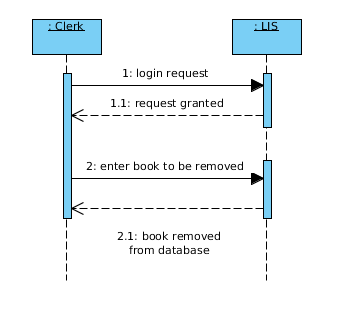
\includegraphics[scale=0.50]{images/seqDiagBookRemoval.png}
\\
The user needs to successfully login to search if a book is present in the library.The user needs to give the details of the book in the system and it will notify about the prescence of the book in the library.

\section{Collaboration Diagram}

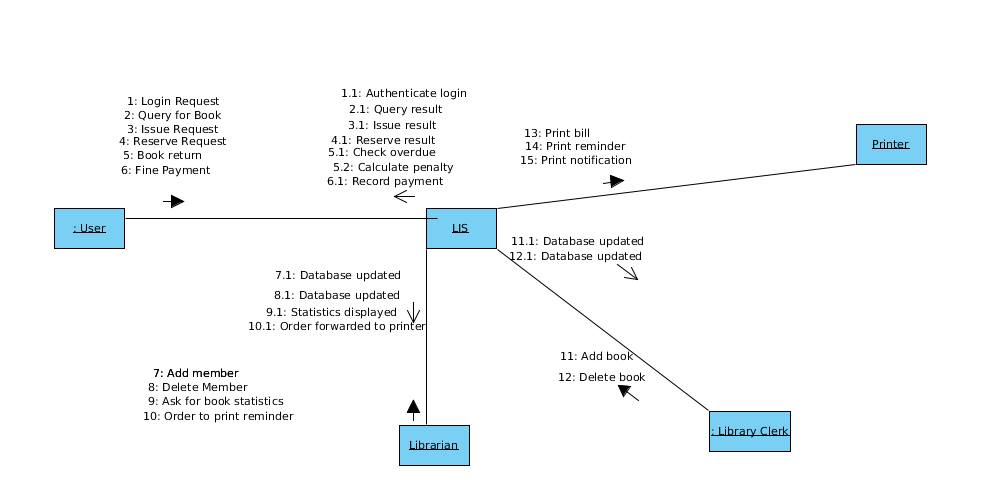
\includegraphics[scale=0.50]{images/collaDiag.jpg}
\\
Description : The user send a specific set of requests to the LIS system like the login request , issue request , return request , serach request and penalty/fine payment.The LIS is bound to send back suitable return messages in case of each of the request messages sent ot the system.
\\
The library clerk has the priviledge of adding and removing books from the system and the LIS system will automatically update its database inside by a cron job.
\\
The librarian has the sole administrator access to the software and the priviledge of adding a member as well as removing his record from the library.The librian can acces the user details or the history of any user.He can also take a alook into the statistics of any book that is can see the book history and can send a notification to remove a book to the library clerk in case the book has been unused and unissued for a long period of time.
\\
The printer is also linked with the sytem and is used to print the notification and the penalty bills and reminder notifications

\section{Statechart Diagram}

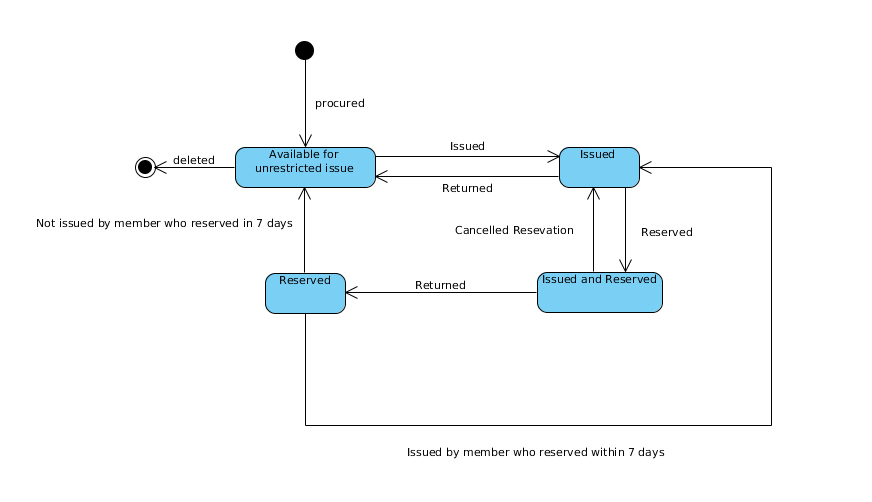
\includegraphics[scale=0.50]{images/stateDiagIssue.png}
\\
Description : The book is avilable for unrestricted issue if it has not been reserved or enen it has been then the user who has reserved it has not issued it within the 7 days afer the notification that the book is available. The book is issued and returned in a separate state. There is also a facility to cancel a reservation .Even after issuing the book may be reserved by some other user. The transition between the states have been clearly shown and demarcated in the above diagram

\section{Activity Diagram}
\subsubsection*{Issue Book Activity Diagram}
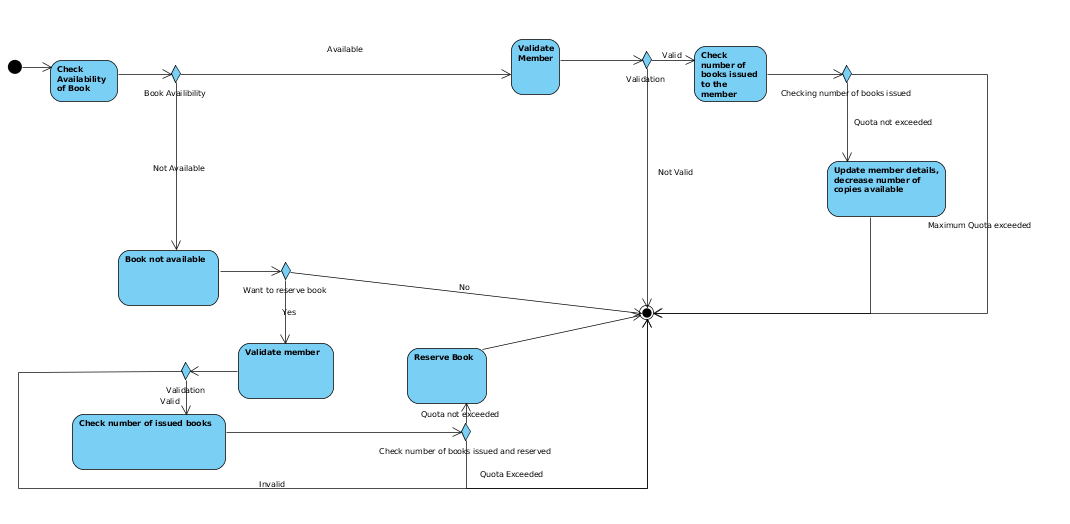
\includegraphics[scale=0.50]{images/activityDiagIssue.png}
\\
Description : First after succesful login the member has to check the availability of the book.We then check if the user is still allowed to issue books or if he has exceeded the maximum book count against his/her account.In case the book is avilable then the book is iisued and the required changes are made to his/her respective account. In case the book is not available then the user can decide to reserve the book or not.If he reserves the book then again we validate him and take a note of the reservation made.A notification will be made to him when the book will be available in the library
\subsubsection*{Return Book Activity Diagram}
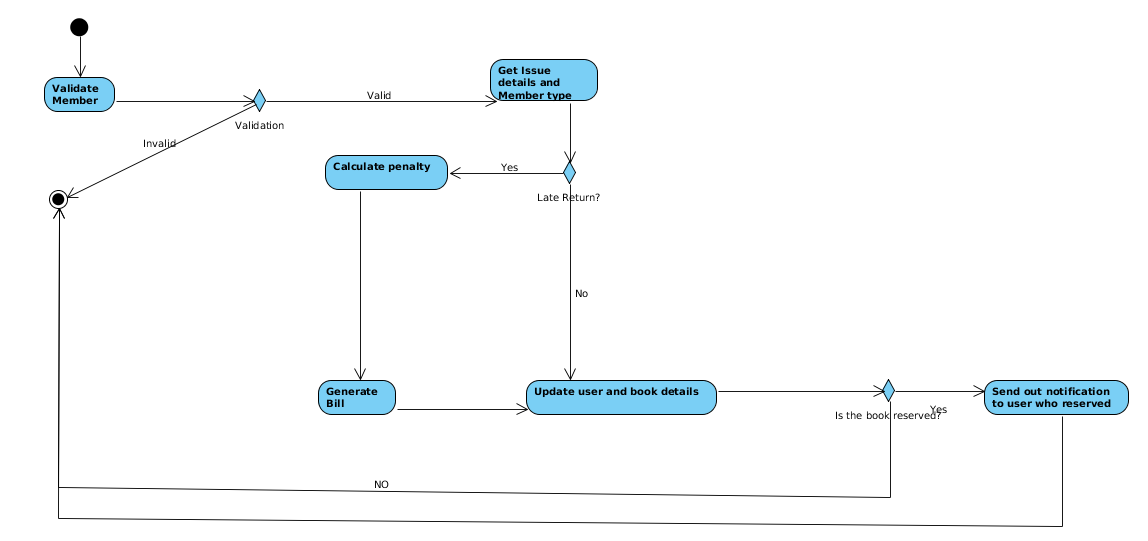
\includegraphics[scale=0.40]{images/activityDiagReturn.png}
\\
Description : We first check for the validation of the member. If the member succesfully logs into his/her account then we ask for the book to be returned. The time for the issue is then checked and using that the number of days he book has been kept is calculated. If trhe book has been kept for a longer period of time than it was meant to be the member or the user is liable to pay fines as per the rate predecided.The fine is calculated by a base on the time the book has been overdue.In any case the book is returned and required updation is donw on the account of the user.
\subsubsection*{Search Book Activity Diagram}
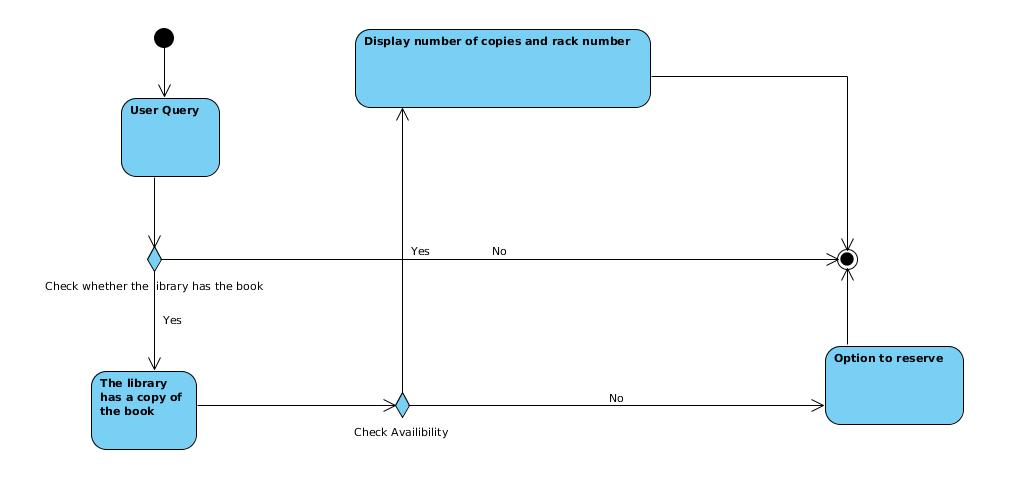
\includegraphics[scale=0.50]{images/activityDiagSearch.jpg}
\\
Description : The user may not need to validate into the system that is the search feature is kept as a global access feature. The person needs to put in the details of the book required in the search field to search for its availability. If the book is present the software will diplay the number of the copies along with their respective rack number for easy access else it will diplay that the book is not currently available.

\section{Data Flow Diagram}

\begin{itemize}
\item Context Diagram\\
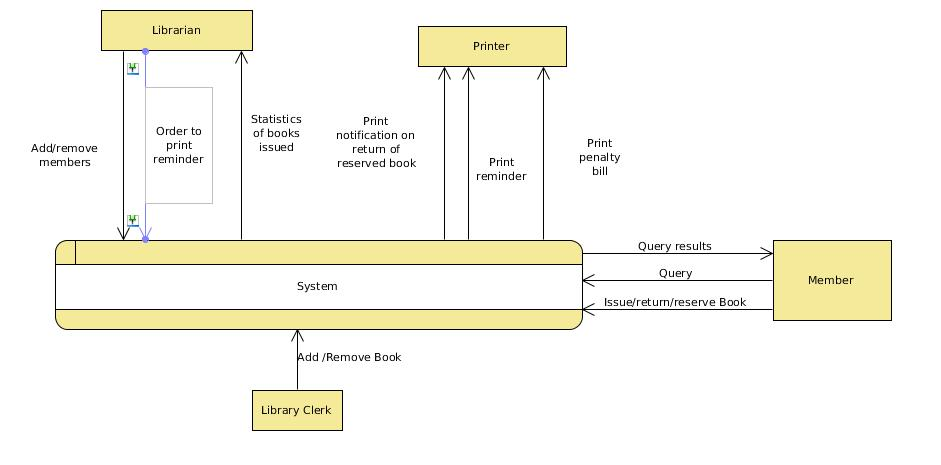
\includegraphics[scale=0.5]{images/contextDiag.jpg}
\item Level 1 DFD\\
\begin{itemize}
\item Diagram for login : \\
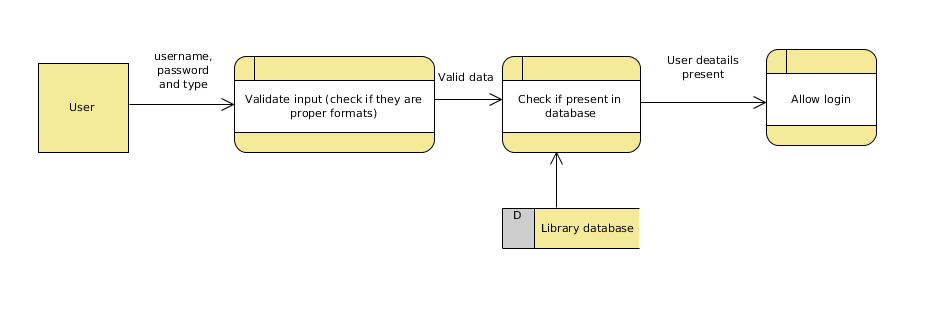
\includegraphics[scale=0.5]{images/dfdDiagLogin.png}\\
\item Diagram for issuing books : \\ 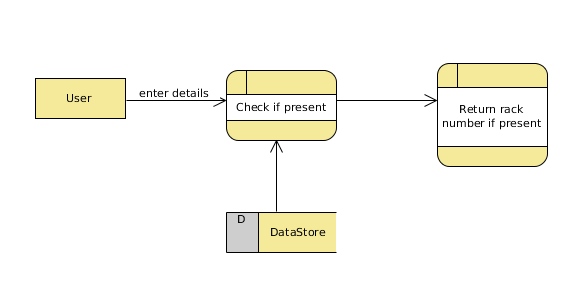
\includegraphics[scale=0.5]{images/DFDDiagIssue.png}\\
\item Diagram for returning books : \\ 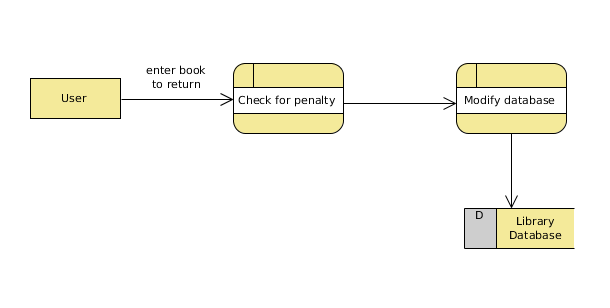
\includegraphics[scale=0.5]{images/dfdDiagReturnBook.png}\\
\item Diagram for searching books : \\ 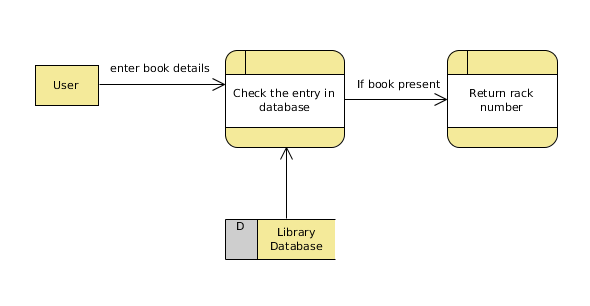
\includegraphics[scale=0.5]{images/dfdDiagSearch.png}\\
\end{itemize}
\end{itemize}

\end{document}